

% Summary Electrodynamics D-ITET
% ===========================================================================
% @Author: Noah Huetter
% @Date:   2019-02-20 17:26:28
% @Last Modified by:   Noah Huetter
% @Last Modified time: 2019-02-24 17:29:55
% ---------------------------------------------------------------------------

\documentclass[a4paper, fontsize=8pt, landscape, DIV=1]{scrartcl}
\usepackage{lastpage}
\usepackage{hyperref}
\usepackage{wrapfig}
% Include general settings and customized commands
%
% General packages and settings
% ===========================================================================
% Author:			Silvano Cortesi (cortesis@student.ethz.ch)
% Version:			1.2
% Last changed:		03.01.2018
%
% ---------------------------------------------------------------------------




\usepackage[german]{babel} %choose your language \usepackage[german]{babel}
%\usepackage[T1]{fontenc}
\usepackage[utf8]{inputenc}
\usepackage{fancyhdr}
%\usepackage{lastpage}
%\usepackage{lmodern}
\usepackage{enumerate}
%\usepackage{float} % for positioning of figures
\usepackage[landscape, margin=1cm]{geometry}
\usepackage[dvipsnames]{xcolor}
\usepackage{pdfpages}


%% Math %%
\usepackage{todonotes}
\usepackage{amscd}
\usepackage{blindtext}
\usepackage{enumitem}
\usepackage{multicol}
\usepackage{parskip}
\usepackage{empheq}
\usepackage{amsmath}
\usepackage{amsfonts}
\usepackage{amssymb}
\usepackage{amsthm}
%\usepackage{dsfont}
%\usepackage{esint} % provides \oiint
\usepackage{mathrsfs}
%\usepackage{trfsigns}
%\numberwithin{equation}{subsection}
%\usepackage{numprint}

%% Graphics & Charts %%
\usepackage{graphicx}
%\usepackage{pdfpages}
%\usepackage{booktabs}
\usepackage{array}
%\usepackage{paralist}
%\usepackage{framed}
%\usepackage{trfsigns}
\usepackage{tikz}
%\usepackage[lofdepth,lotdepth]{subfig}
%\usepackage{tikz}  %Graphen zeichnen
%\usetikzlibrary{decorations.pathmorphing}
%\usetikzlibrary{arrows.meta,arrows}
%\usepackage{pgfplots}
%% General Settings %%
%\setlength{\parindent}{0px}
%\setkomafont{captionlabel}{\normalfont\bfseries}

%\pagestyle{fancy}
%\lfoot{\tiny \today}
%\rfoot{\thepage\  / \pageref{LastPage}}
%\cfoot{}
%\renewcommand{\footrulewidth}{0.4pt}

%% provides command \uline{} for underlining words
%\usepackage{ulem}

%% colour headings
%\usepackage{color}
%\definecolor{bluen}{cmyk}{1,0.5,0,0}
%\definecolor{bloodorange}{cmyk}{0,.92,1,.2}
%\addtokomafont{section}{\color{bloodorange}}
%\addtokomafont{subsection}{\color{bloodorange}}
%\addtokomafont{subsubsection}{\color{bloodorange}}
%\addtokomafont{paragraph}{\small\color{bloodorange}}
%\addtokomafont{subparagraph}{\small\color{bloodorange}}

%% Signs & Special Formating %%
%\usepackage{ulem} %normalem: \emph{Text} is italic again.
%\usepackage{multicol,multirow}
%\usepackage{tabularx}
%\usepackage{stackrel}
%\usepackage{makeidx}
%\usepackage{mparhack} % bessere margiale bei seitenumbruch

% make document compact
\usepackage[compact]{titlesec}
\titlespacing{\section}{0pt}{*0}{*0}
\titlespacing{\subsection}{0pt}{*0}{*0}
\titlespacing{\subsubsection}{0pt}{*0}{*0}

\parindent 0pt
\pagestyle{empty}
\setlength{\unitlength}{1cm}
\setlist{leftmargin = *}

%include also newer PDF
\pdfminorversion=6

% Set the color of your style
% Avaiable are: Apricot, Aquamarine, Bittersweet, Black, Blue, blue, BlueGreen, BlueViolet, BrickRed, Brown, BurntOrange, CadetBlue, CarnationPink, Cerulean, CornflowerBlue, Cyan, Dandelion, DarkOrchid, Emerald, ForestGreen, Fuchsia, Goldenrod, Gray, Green, GreenYellow, JungleGreen, Lavender, ... (more at: http://en.wikibooks.org/wiki/LaTeX/Colors)
\def\StyleColor{MidnightBlue}

%
% General commands
% ===========================================================================
% Author:			Silvano Cortesi (cortesis@student.ethz.ch)
% Version:			1.2
% Last changed:		03.01.2018
%
% ---------------------------------------------------------------------------

%..ROEMISCHE_ZAHLEN
	\newcommand{\Roe}[1]{\uppercase\expandafter{\romannumeral #1 }}

%..ZAHLENMENGEN
	\newcommand{\N}{\mathbb{N}}
	\newcommand{\Z}{\mathbb{Z}}
	\newcommand{\Q}{\mathbb{Q}}
	\newcommand{\R}{\mathbb{R}}
	\newcommand{\real}{\R}
	\newcommand{\C}{\mathbb{C}}
	\newcommand{\complex}{\C}
	\newcommand{\0}{\mathbb{O}}
	\newcommand{\F}{\mathbb{F}}
	\newcommand{\K}{\mathbb{K}}
    \newcommand{\angstrom}{\textup{\AA}}
    
%..PFEILE
	\renewcommand{\leadsto}{\Longrightarrow}
	\newcommand{\leftrightleadsto}{\Longleftrightarrow}

%..VEKTOREN
	\newcommand{\Ul} {\underline}
	\newcommand{\vEx} {\vec{e}_x}
	\newcommand{\vEy} {\vec{e}_y}
	\newcommand{\vEz} {\vec{e}_z}
	\newcommand{\vEq} {\vec{e_1}}
	\newcommand{\vEw} {\vec{e_2}}
	\newcommand{\vEe} {\vec{e_3}}
	\newcommand{\transpose} {^{\text{T}}}
	\newcommand{\vect}[1]{\boldsymbol{#1}}
	
%..MATRIX
    \newcommand{\MATR}[1]{ \displaystyle \left( \begin{matrix} #1 \end{matrix} \right)}
    \newcommand{\MATRABS}[1]{ \displaystyle \left| \begin{matrix} #1 \end{matrix} \right|}

%..GRAPHICS
  \newcommand{\cgraphic}[2]{\begin{center}\includegraphics[width=#1\columnwidth,keepaspectratio]{#2}\end{center}}
  
%..FONTS AND LETTERS
  \newcommand*{\rom}[1]{\uppercase\expandafter{\romannumeral #1\relax}}

%..KOMPLEXE ZAHLEN
	\renewcommand{\Re}{\text{Re}\,}
	\renewcommand{\Im}{\text{Im}\,}

%..OPERATOREN
	\DeclareMathOperator{\grad}{grad}
	\renewcommand{\div}{\text{div}\,}
    	\DeclareMathOperator{\rot}{rot}
    	\DeclareMathOperator{\divg}{div}
    	\DeclareMathOperator{\Tr}{Tr}
    	\DeclareMathOperator{\const}{const}
	\DeclareMathOperator{\imag}{i}
	\newcommand{\Lapl}{\hbox{\footnotesize{$\Delta$}}}

%..DIFFERENTIALRECHNUNG
	\newcommand{\Dx} {\,\mathrm{d}}
	\newcommand{\abl}[1] {\frac{\mathrm{d}}{\mathrm{d}#1}}
	\newcommand{\Abl}[2] {\frac{\mathrm{d}#1}{\mathrm{d}#2}}
	\newcommand{\ablq}[1] {\frac{\mathrm{d^2}}{\mathrm{d}#1^2}}
	\newcommand{\Ablq}[2] {\frac{\mathrm{d^2}#1}{\mathrm{d}#2^2}}
	\newcommand{\pabl}[1] {\frac{\partial}{\partial#1}}
	\newcommand{\pablq}[1] {\frac{\partial^2}{\partial#1^2}}
	\newcommand{\Pabl}[2] {\frac{\partial#1}{\partial#2}}
	\newcommand{\Pablq}[2] {\frac{\partial^2#1}{\partial#2^2}}

%..INTEGRALRECHNUNG
	\newcommand{\dint}{\displaystyle{\int}}
	\newcommand{\intab}{\int^b_a}
	\newcommand{\intinf}{\int_{-\infty}^\infty}
	\newcommand{\dintab}{\displaystyle{\int^b_a}}
	\newcommand{\dintpi}{\displaystyle{\int^{\pi}_{-\pi}}}
	\newcommand{\dintzpi}{\displaystyle{\int^{2\pi}_{\mbox{-}2\pi}}}
	\newcommand{\dA}{\hspace{4pt}\mathrm{d}A}
	\newcommand{\dx}{\hspace{4pt}\mathrm{d}x}
	\newcommand{\dy}{\hspace{4pt}\mathrm{d}y}
	\newcommand{\dz}{\hspace{4pt}\mathrm{d}z}
	\newcommand{\dr}{\hspace{4pt}\mathrm{d}r}
	\newcommand{\ds}{\hspace{4pt}\mathrm{d}s}
	\newcommand{\dS}{\hspace{4pt}\mathrm{d}S}
	\newcommand{\dt}{\hspace{4pt}\mathrm{d}t}
	\newcommand{\dm}{\hspace{4pt}\mathrm{d}m}
	\newcommand{\dk}{\hspace{4pt}\mathrm{d}k}
	\newcommand{\dl}{\hspace{4pt}\mathrm{d}l}
	\newcommand{\du}{\hspace{4pt}\mathrm{d}u}
	\newcommand{\dv}{\hspace{4pt}\mathrm{d}v}
	\newcommand{\dV}{\hspace{4pt}\mathrm{d}V}
	\newcommand{\dphi}{\hspace{4pt}\mathrm{d}\varphi}
	\newcommand{\domega}{\hspace{4pt}\mathrm{d}\omega}
	\newcommand{\dvarsigma}{\hspace{4pt}\mathrm{d}\varsigma}
	\newcommand{\dtau}{\hspace{4pt}\mathrm{d}\tau}
	\newcommand{\dtheta}{\hspace{4pt}\mathrm{d}\vartheta}
	\newcommand{\dmu}{\hspace{4pt}\mathrm{d}\mu}
	\newcommand{\dxi}{\hspace{4pt}\mathrm{d}\xi}
	\newcommand{\deta}{\hspace{4pt}\mathrm{d}\eta}
	\newcommand{\dvecl}{\hspace{4pt}\mathrm{d}\vec{l}}
	\newcommand{\dvecS}{\hspace{4pt}\mathrm{d}\vec{S}}

%..LIMES
    \DeclareMathOperator{\limni}{\lim\limits_{n\to\infty}}
    \DeclareMathOperator{\limxi}{\lim\limits_{x\to\infty}}
    \DeclareMathOperator{\limho}{\lim\limits_{h\to0}}
    \newcommand{\limxai}[1]{\ensuremath{\lim\limits_{x\to #1}}}

%..SUMMEN
    \DeclareMathOperator{\sumni}{\sum_{n=0}^{\infty}}
    \newcommand{\sumnia}[1]{\ensuremath{\sum_{n=#1}^{\infty}}}


%..PARTIELLE ABLEITUNG
    \DeclareMathOperator{\partf}{\dfrac{\partial f}{\partial x}}
    \newcommand{\partfo}[1]{\ensuremath{\dfrac{\partial f}{\partial #1}}}
    \newcommand{\parto}[1]{\ensuremath{\dfrac{\partial }{\partial #1}}}
    \newcommand{\partt}[2]{\ensuremath{\dfrac{\partial^2 }{\partial #1\partial #2}}}
    \newcommand{\partq}[1]{\ensuremath{\dfrac{\partial^2 }{\partial #1^2}}}


%..ENUMERATION
    \newenvironment{abc}{\begin{enumerate}[(a)]}{\end{enumerate}}
    \newenvironment{cabc}{\begin{compactenum}[(a)]}{\end{compactenum}}
    \newenvironment{romanenum}{\begin{enumerate}[i.]}{\end{enumerate}}
    \newenvironment{cromanenum}{\begin{compactenum}[i.]}{\end{compactenum}}

%..FUNCTIONS
    \DeclareMathOperator{\arsinh}{arsinh}
    \DeclareMathOperator{\arcosh}{arcosh}
    \DeclareMathOperator{\artanh}{artanh}
    \DeclareMathOperator{\arcoth}{arcoth}
    \DeclareMathOperator{\arccot}{arccot}
    \DeclareMathOperator{\Arg}{Arg}
    \DeclareMathOperator{\Log}{Log}
    \newcommand{\dis}[1]{\hspace{#1cm}}
    \newcommand{\abs}[1]{\ensuremath{\left\vert#1\right\vert}}
    \newcommand{\attention}{\raisebox{-1pt}{{\makebox[1.6em][c]{\makebox[0pt][c]{\raisebox{.13em}{\small!}}\makebox[0pt][c]{\color{red}\Large$\bigtriangleup$}}}}}
    \DeclareMathOperator{\meq}{\stackrel{!}{=}}
    
    
% section color box
\setkomafont{section}{\mysection}
\newcommand{\mysection}[1]{%
    \Large\sffamily\bfseries%
    \setlength{\fboxsep}{0cm}%already boxed
    \colorbox{\StyleColor!40}{%
        \begin{minipage}{\linewidth}%
            \vspace*{2pt}%Space before
            #1
            \vspace*{-1pt}%Space after
        \end{minipage}%
    }}

%subsection color box
\setkomafont{subsection}{\mysubsection}
\newcommand{\mysubsection}[1]{%
    \normalsize \sffamily\bfseries%
    \setlength{\fboxsep}{0cm}%already boxed
    \colorbox{\StyleColor!20}{%
        \begin{minipage}{\linewidth}%
            \vspace*{2pt}%Space before
             #1
            \vspace*{-1pt}%Space after
        \end{minipage}%
    }}

% highlighter
\newcommand{\hilight}[1]{\colorbox{\StyleColor}{#1}}
\newcommand{\highlighty}[1]{%
  \setlength{\fboxsep}{0pt}\colorbox{yellow!100}{\ensuremath{#1}}}

\newcommand{\highlightg}[1]{%
  \setlength{\fboxsep}{0pt}\colorbox{green!100}{\ensuremath{#1}}}

\newcommand{\highlightbg}[1]{%
   \colorbox{green!100}{$\displaystyle #1$}}  

% equation box        
\newcommand{\eqbox}[1]{\setlength{\fboxrule}{1mm}\fcolorbox{\StyleColor}{white}{\hspace{0.5em}$\displaystyle#1$\hspace{0.5em}}}

%center equationbox
\newcommand{\ceqbox}[1]{\vspace*{4pt} \begin{center}\eqbox{#1}\end{center}\vspace*{4pt}}

%change page style for header
\pagestyle{fancy}
\footskip 20pt


% -----------------------------------------------------------------------
\IfFileExists{../build/revision.tex}{
  \input{../build/revision.tex}
  \rhead{Compiled: \compiledate \hspace{1em} Commit: \revision \hspace{1em} Noah Huetter}
}{\rhead{Noah Huetter}}

\lhead{ETH Electrodynamics}
\chead{\thepage}
\cfoot{}
\headheight 17pt \headsep 10pt
\title{ETH Electrodynamics}
\author{Noah Huetter}

\date{\today}
\begin{document}

\setcounter{secnumdepth}{2} %no enumeration of sections
\begin{multicols*}{4}
	\section*{Disclaimer}
	This summary is part of the lecture ``Electrodynamics'' by Prof. Dr. L. Novotny (FS19). It is based on the lecture. \\[6pt]
	Please report errors to \href{mailto:huettern@student.ethz.ch}{huettern@student.ethz.ch} such that others can benefit as well.\\[6pt]	
  The upstream repository can be found at \href{https://github.com/noah95/formulasheets}{https://github.com/noah95/formulasheets}
	\vfill\null
	\pagebreak
  \maketitle 
  \thispagestyle{fancy}

  % ---------------------------------------------------------------------------
  \section{Conventions}
  % ---------------------------------------------------------------------------
  \begin{tabular}[h]{l l}
    $V$ & Volume \\
    $dV$ & infinitesimal volume elements \\
    $A$ & surface \\
    $da$ & infinitesimal surface elements \\
    $ds$ & infinitesimal line element \\
    $\partial V$ & closed surface of the volume $V$ \\
    $\partial A$ & circumference of area $A$ \\
    $\mbf{n}$ & unit vector normal to suface / circumference \\
    $\rho$ & Charge density \\
    $\mbf{j}$ & Current density \\
    $\mbf{E}$ & Electric field \\
    $\mbf{H}$ & Magnetic field \\
    $\mbf{D}$ & Displacement \\
    $\mbf{M}$ & Magnetization \\
    $\phi$ & Electric potential
  \end{tabular}
  % ---------------------------------------------------------------------------
  \section{Mathematics}
  % ---------------------------------------------------------------------------
    \subsection{Linear Algebra}

    \[\nabla = \MATR{\pabl{x}\\\pabl{y}\\\pabl{z}} \]
    
    \subsubsection{Rotation}
    The cross product of the nabla operator and the vector field $\vec{F}$
    \[ \nabla \times \vec{F} = \det \MATR{\vEx & \vEy & \vEz \\ \pabl{x} & \pabl{y} & \pabl{z} \\ \vec{F}_x&\vec{F}_y&\vec{F}_z} = \MATR{\pabl{y}\vec{F}_z - \pabl{z}\vec{F}_y \\ -\pabl{x}\vec{F}_z + \pabl{z}\vec{F}_x \\ \pabl{x}\vec{F}_y - \pabl{y}\vec{F}_x } \]

    \subsubsection{Divergence}
    \[\nabla \cdot \vec{F} = \pabl{x}F_x + \pabl{y}F_y + \pabl{z}F_z = \div(\vec{F})\]

    \subsubsection{Combination}
    Always solve right to left.
    \[ \nabla \times \nabla \phi(\vec{r}) = \nabla \times(\nabla\phi(\vec{r})) = \dots = 0 \]
    \[\nabla\cdot\nabla\times\vec{F} = \nabla\cdot(\nabla\times\vec{F}) = \dots = 0\]
    Rotation of rotation:
    \[\nabla\times\nabla\times\vec{F} = \nabla{\nabla\cdot\vec{F}}-\nabla^2\vec{F}\]

    \subsection{Integrals}
    \subsubsection{Line integral inside Vector Field}
    \begin{enumerate}
      \item Parametrize curve with $t$. Split integral if necessary for differenc parametrizations
       \begin{align*} x&:f(t) & y&:f(t) & z&:f(t)\end{align*}
      \item Calcualate derivative of normal vector along curve
      \begin{align*}\Abl{\vec{s}}{t} &= x'(t)\vEx+y'(t)\vEy+z'(t)\vEz \\ \Dx \vec{s} &= \MATR{x'(t)\\y'(t)\\z'(t)}\Dx t\end{align*}
      \item Solve integral
      \[ \int_{\partial A} F(\vec{r}) \Dx \vec{s} = \intab F(x(t),y(t),z(t)) \cdot \MATR{x'(t)\\y'(t)\\z'(t)}\Dx t \]
    \end{enumerate}

    \subsection{Stokes' Therorem}
    \begin{center}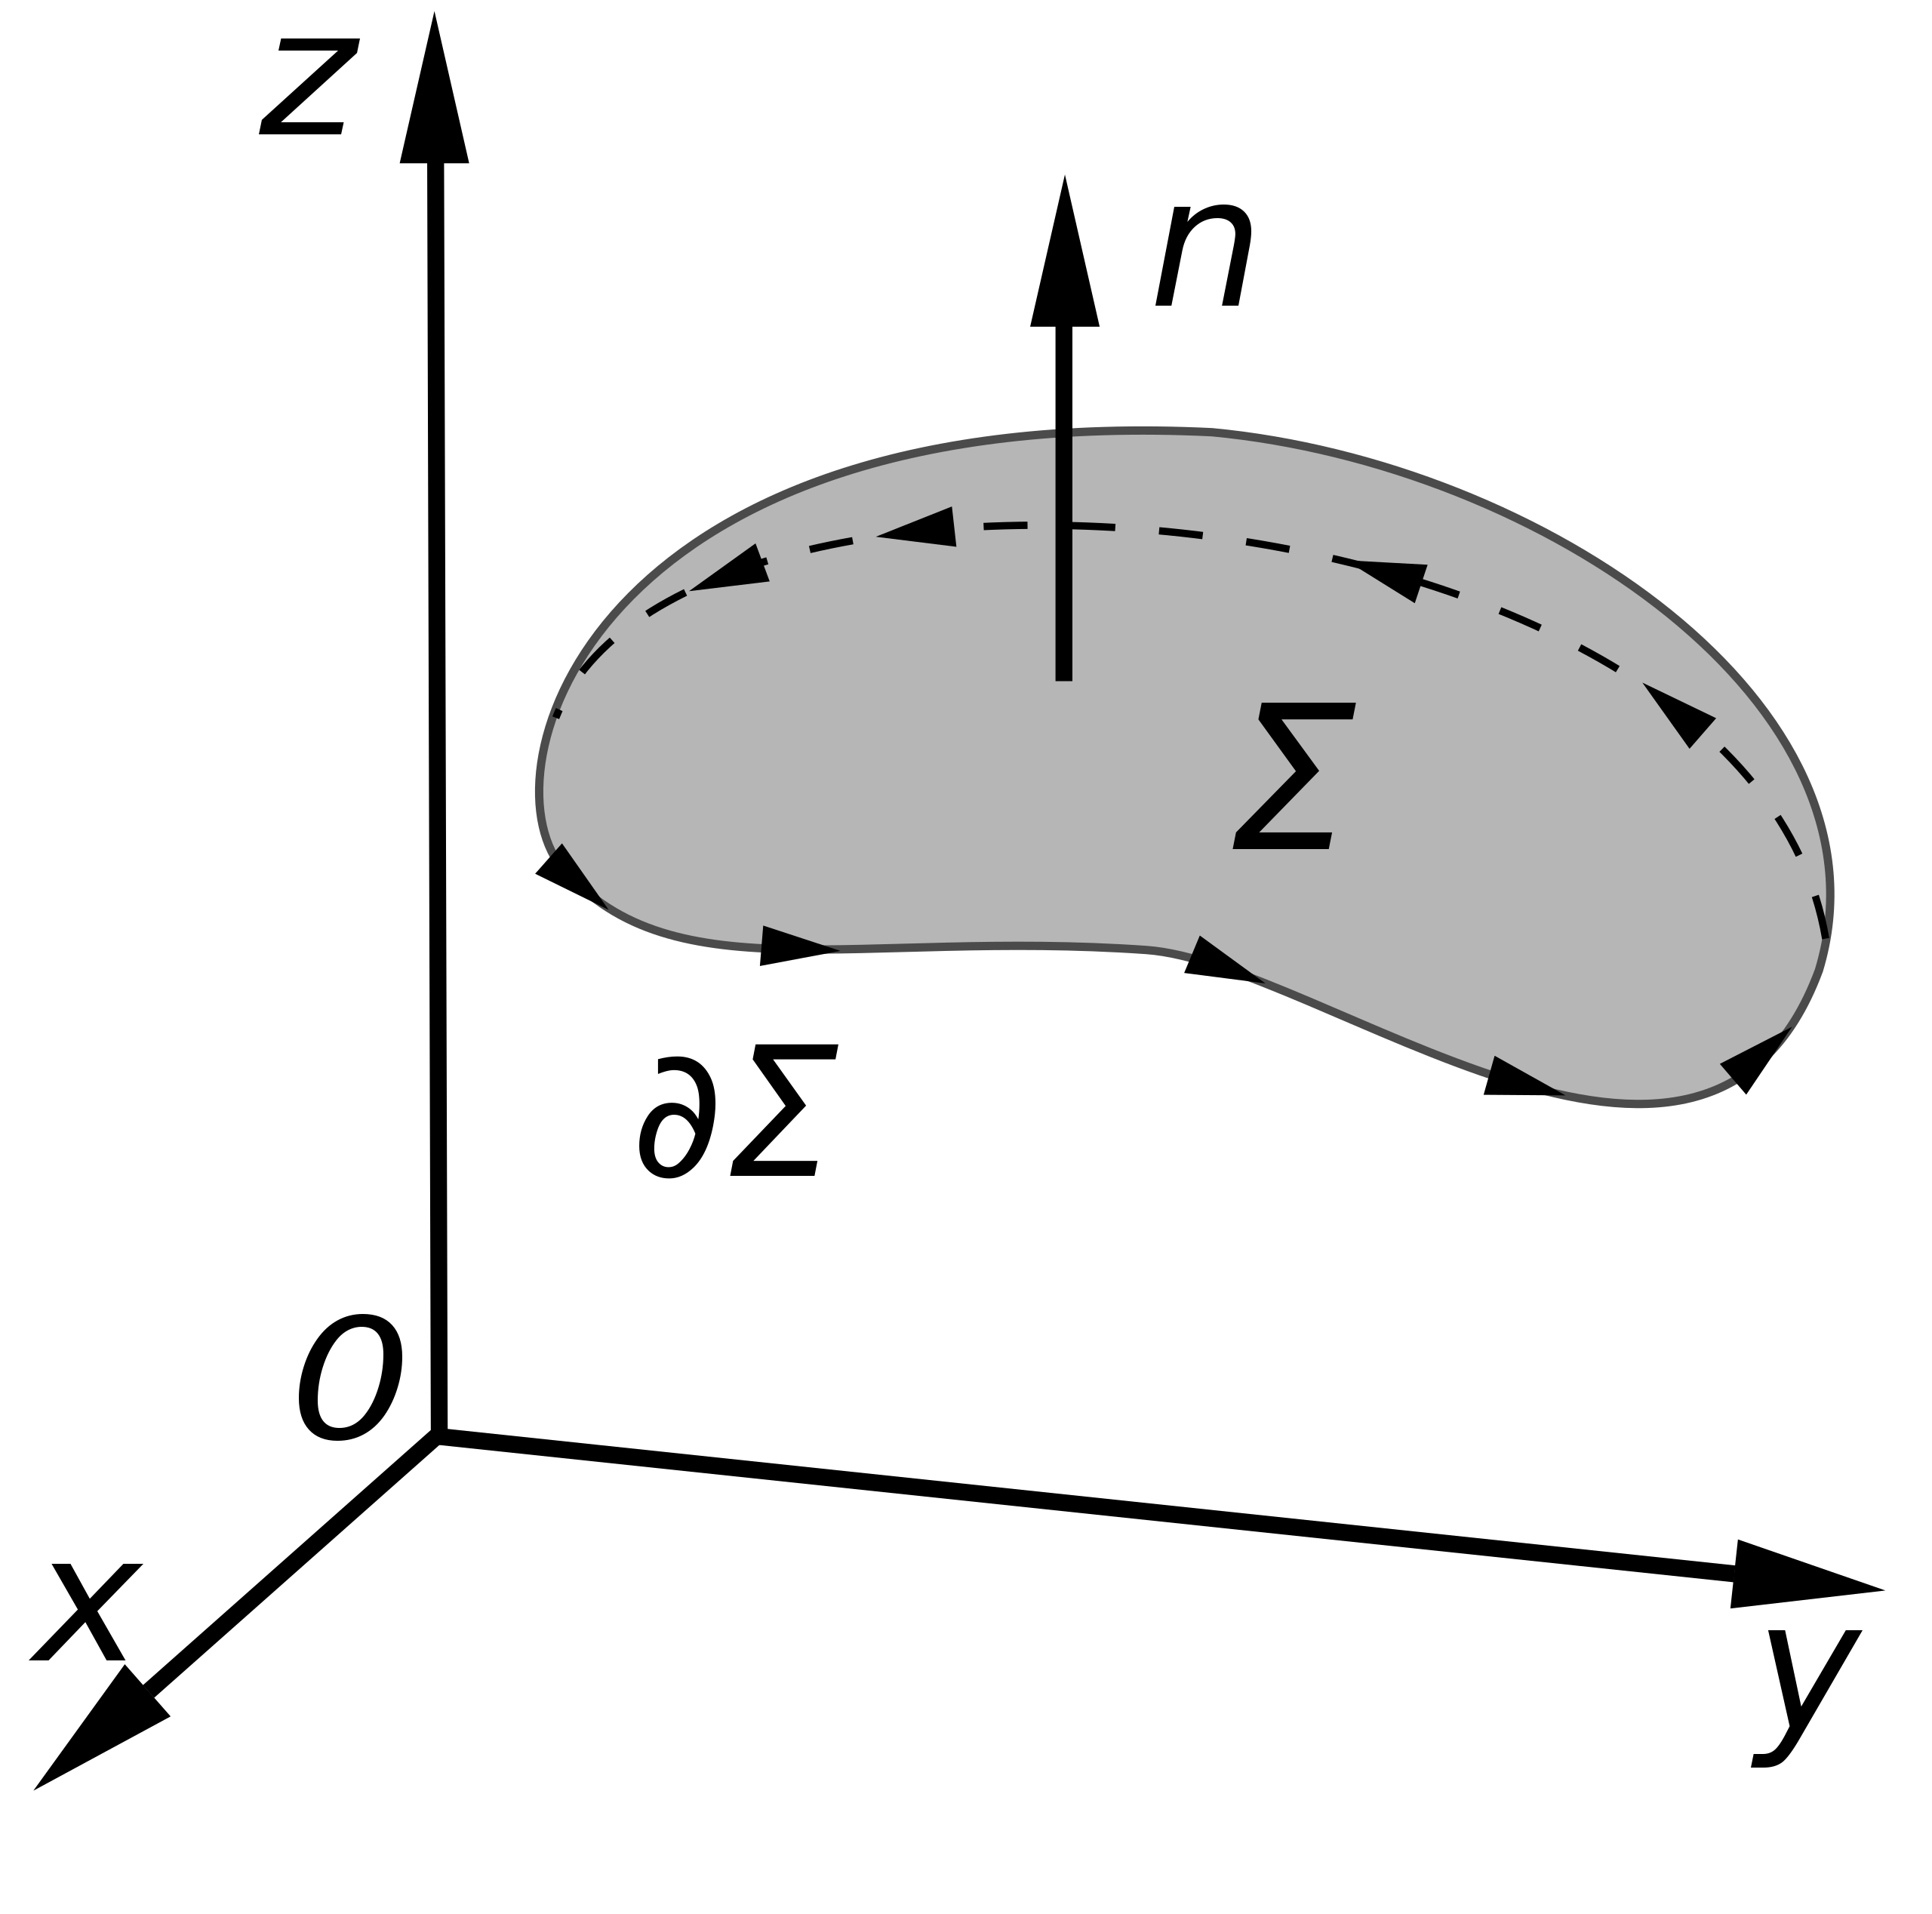
\includegraphics[width=0.5\columnwidth,keepaspectratio]{img/stokes.png}\end{center}
    \[\int_{\partial A}F(\vec{r})\Dx \vec{s} = \int_A[\nabla\times F(\vec{r})]\cdot\vec{n}\Dx a\]
    The sum of flux along the contour $\partial A$ in contour direction is the same as the sum of curl $\nabla\times \vec{F}$ in normal direction $\vec{n}$ on the area $A$.

    

    \subsection{Gauss Therorem}
    Also known as divergence theorem.
    \begin{center}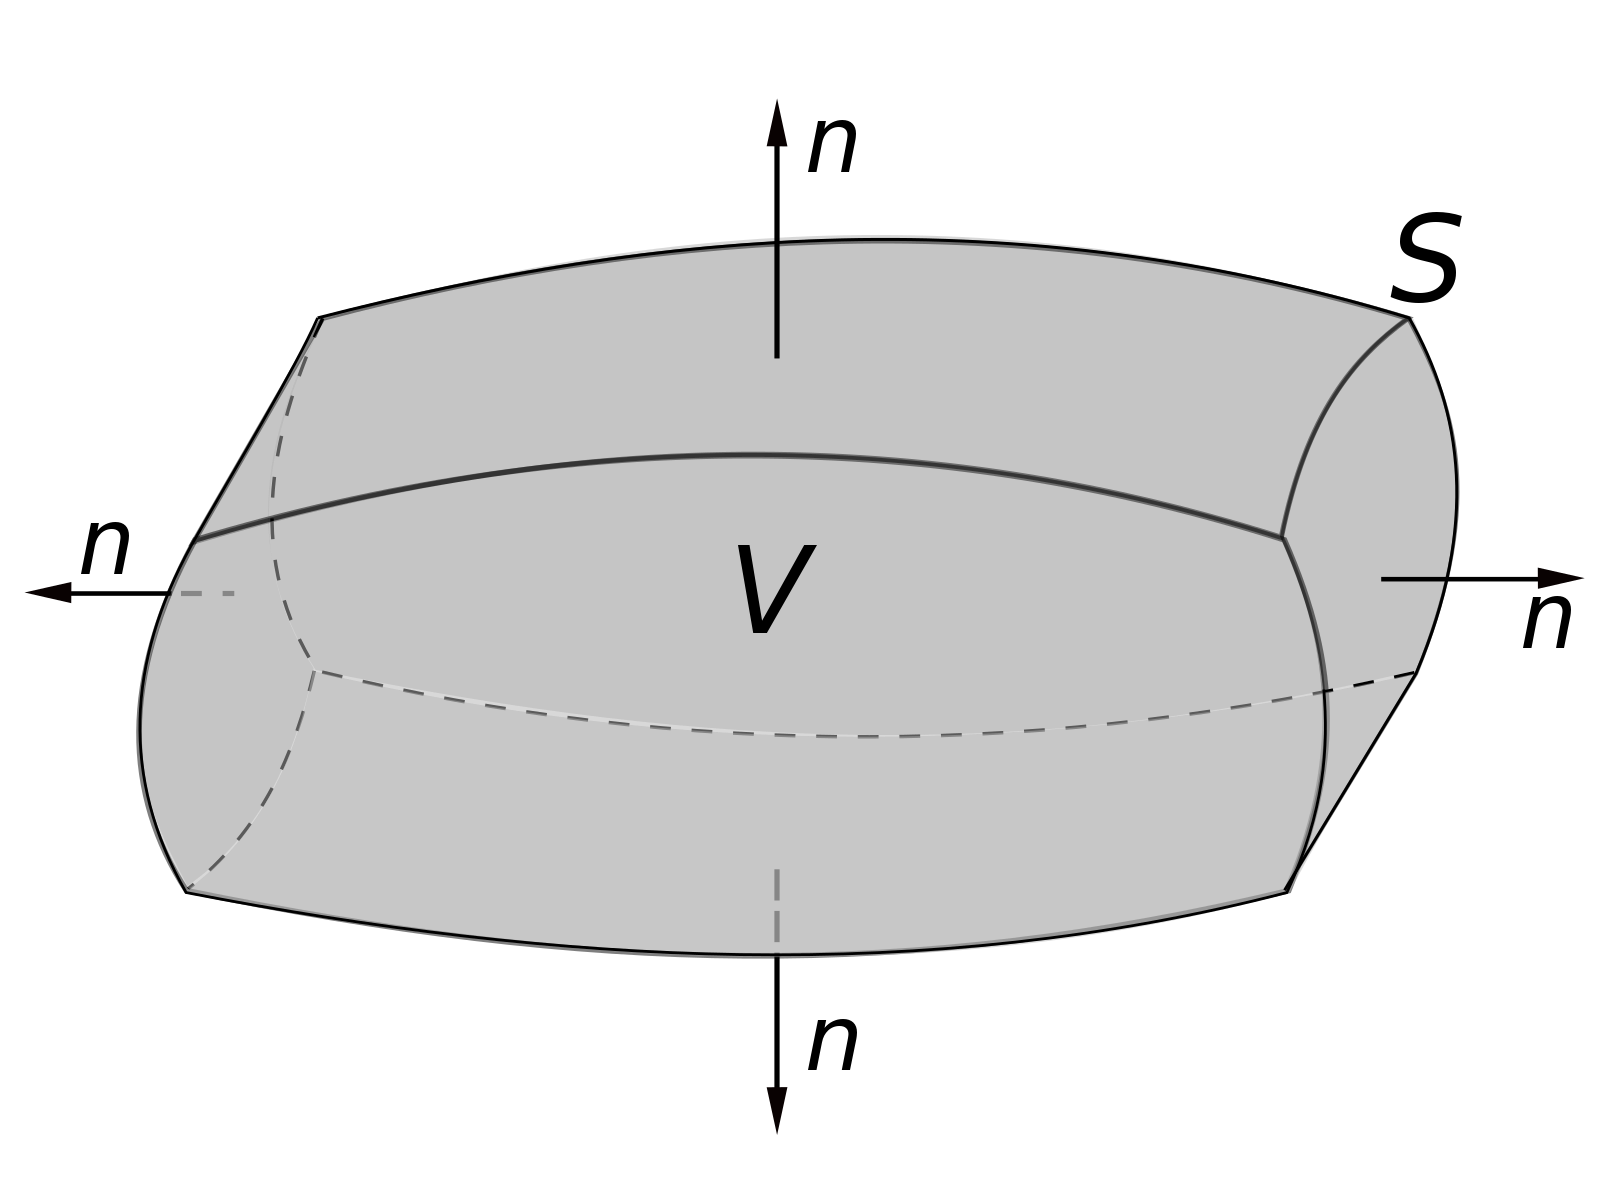
\includegraphics[width=0.5\columnwidth,keepaspectratio]{img/gaussthm.png}\end{center}
    \[ \int_{\partial V} \vec{F}(\vec{r})\cdot\vec{n}\Dx a = \int_V \nabla\vec{F}(\vec{r})\Dx V \]
    Sum of flux across surface $\partial A$ in normal direction $\vec{n}$ is the same as the sum of divergence inside the region $V$.

  % ---------------------------------------------------------------------------
  \section{Pre-Maxwellian Electrodynamics}
  % ---------------------------------------------------------------------------
  \subsubsection{Gauss' Law}
  The net flux through a surface is equal to $1/\epsilon_0$ times the net electric charge within that surface.
  \cgraphic{0.5}{img/gausslaw.png}
  \[\int_{\partial V}\mbf{E}(\mbf{r},t)\cdot \mbf{n} \Dx a = \frac{1}{\epsilon_0}\int_V\rho(\mbf{r},t)\Dx V \]

  \subsubsection{Faraday's Law}
  The electromotive force around a path is equal to the negative change in time of the magnetic flux enclosed by the path.
  \cgraphic{0.5}{img/faradaylaw.png}
  \[\int_{\partial A}\mbf{E}(\mbf{r},t)\cdot \Dx s = -\frac{\partial}{\partial t}\int_A \mbf{B}(\mbf{r},t)\cdot \mbf{n} \Dx a \]

  \subsubsection{Ampere's Law}
  The magnetic field created by an electric current is proportional to the size of that electric current.
  \cgraphic{0.5}{img/amperelaw.png}
  \[\int_{\partial A}\mbf{B}(\mbf{r},t)\cdot \Dx s = \mu_0 \int_A \mbf{j}(\mbf{r},t)\cdot \mbf{n} \Dx a \]

  \subsubsection{Non-existence of magnetic charges}

  \cgraphic{0.5}{img/magchargnonexistence.png}
  \[\int_{\partial V}\mbf{B}(\mbf{r},t)\cdot \mbf{n} \Dx a = 0 \]
  
  \subsubsection{Kirchhoff}
  Reducing Apere's law to any closed surfece states that the flux of current through any closed surface is zero: What flows in has to flow out.
  \[ \int_{\partial V} \mbf{j}(\mbf{r},t) \cdot \mbf{n}\Dx a = 0 \]

  From Faraday's law if no time-varying magnetic fields are present follows the second Kirchhoff law (Knotenregel):
  \[ \int_{\partial A} \mbf{E}(\mbf{r},t)\cdot \Dx s = 0 \]

  The two Kirchhoff laws form the basis for circuit theory and electronic design.

  % ---------------------------------------------------------------------------
  \section{Maxwell's Equations}
  % ---------------------------------------------------------------------------
  The pre-Maxwellian equations summarize the electromagnetism before Maxwell. In 1873 however, Maxwell introduced a critical modification.

  \subsection{Displacement Current}
  The law that the net flux through a closed surface is zero is flawed. For example: Identical charges released will speed out because of Coulomb repulsion and there will be a net outward current. Kirchhoffs first law has to be corrected as follows:
  \[\int_{\partial V} \mbf{j}(\mbf{r},t) \cdot \mbf{n} \Dx a\]

  \texttt{continuity equation}: The outward current is balanced by the decrease of charge inside the surface.

  \subsection{Maxwell's Equations in Integral Form}
  \begin{align*}
    \int_{\partial V} \mbf{D}(\mbf{r},t) \cdot\mbf{n}\Dx a &= \int_V \rho(\mbf{r},t) \Dx V \\
    \int_{\partial A} \mbf{E}(\mbf{r},t) \cdot \Dx s &= -\frac{\partial}{\partial t}\int_A \mbf{B}(\mbf{r},t) \cdot \mbf{n} \Dx a \\
    \int_{\partial A} \mbf{H}(\mbf{r},t) \cdot \Dx s &= \int_A \left[\mbf{j}(\mbf{r},t) + \frac{\partial}{\partial t}\mbf{D}(\mbf{r},t)\right] \cdot \mbf{n} \Dx a \\
    \int_{\partial V} \mbf{B}(\mbf{r},t) \cdot \mbf{n} \Dx a &= 0
  \end{align*}

  The displacement $D$ and the magnetic field $H$ account for secondary sources through
  \[\mbf{D}(\mbf{r},t) = \epsilon_0 \mbf{E}(\mbf{r},t)+\mbf{P}(\mbf{r},t)\]
  \[ \mbf{B}(\mbf{r},t) = \mu_0 [\mbf{H}(\mbf{r},t) + \mbf{M}(\mbf{r},t)]\]

  \subsection{Maxwell's Equations in Differential Form}
  \begin{align*}
    \nabla \cdot \mbf{D}(\mbf{r},t) &= \rho(\mbf{r},t) \\
    \nabla\times \mbf{E}(\mbf{r},t) &= -\pabl{t}\mbf{B}(\mbf{r},t) \\
    \nabla\times \mbf{H}(\mbf{r},t) &= \pabl{t}\mbf{D}(\mbf{r},t) + \mbf{j}(\mbf{r},t)\\
    \nabla \cdot \mbf{B}(\mbf{r},t) &= 0
  \end{align*}

  % ---------------------------------------------------------------------------
  \section{Electrostatics}
  % ---------------------------------------------------------------------------
  We modify Faraday's law by setting the change of magnetic flux to zero. 
  \[\int_{\partial A}\mbf{E}(\mbf{r},t)\cdot \Dx s = 0 \]

  By applying the theorems of Gauss and Stokes we get the following identities:
  \begin{align*}
    &\nabla \cdot \mbf{E}(\vec{r}) = \frac{1}{\epsilon_0\rho(\vec{r})} & &\nabla\times\mbf{E}(\vec{r}) = 0 \\
    &\mbf{E} = -\nabla\phi & &\nabla^2\phi(\vec{r}) = -\frac{1}{\epsilon_0}\rho(\vec{r})
  \end{align*}

  Combining them we can write the poisson equation:
  \begin{align*}
    \nabla^2\Phi(\vec{r}) &= -\frac{1}{\epsilon_0}\rho(\vec{r}) &
    \phi(\vec{r}) &= \frac{1}{4\pi\epsilon_0}\int\frac{\rho(\vec{r})}{|\vec{r}-\vec{r}'|}\Dx V'
  \end{align*}

  Where $\phi(\vec{r})$ is the electric potential at point $\vec{r}$.
  \cgraphic{0.5}{img/epot.png}

  \subsection{Point Charge}
  E-field of a point charge:
  \cgraphic{0.5}{img/ptcharge.png}
    \[\int_{\partial A} \vec{E}\vec{n} \Dx a = E\cdot4\pi r^2 = \frac{q}{\epsilon_0} \]
  \begin{align*}
    \vec{E} &= \frac{1}{4\pi\epsilon_0}\frac{q}{r^2}\vec{n}_r & \vec{E}&=-\nabla\phi & \phi&=\frac{1}{4\pi\epsilon_0}\frac{q}{r}
  \end{align*}



\end{multicols*}

\setcounter{secnumdepth}{2}
\end{document}
